\documentclass[11pt,a4paper]{article}
\usepackage[T1]{fontenc}
\usepackage[utf8]{inputenc}
\usepackage{lmodern}
\usepackage{amsmath,amssymb}
\usepackage{geometry}
\usepackage{graphicx}
\usepackage{float}
\usepackage{booktabs}
\usepackage{array}
\usepackage{longtable}
\usepackage{tabularx}
\usepackage{caption}
\usepackage[hidelinks]{hyperref}
\usepackage{setspace}
\usepackage{xcolor}
\usepackage{enumitem}
\graphicspath{{../figures/}{../figures/}}
\geometry{a4paper, margin=0.82in}
\setstretch{1.04}
\captionsetup{font=small,labelfont=bf}
\setlist[itemize]{leftmargin=1.35em}
\setlist[enumerate]{leftmargin=1.35em}
\newcommand{\dAIC}{\Delta\mathrm{AIC}}
\newcommand{\rrf}{\mathrm{RRF}}
\newcommand{\snrrf}{\mathrm{SN\mbox{-}RRF}}
\newcommand{\vout}{v_{\mathrm{outer}}}
\newcommand{\rlast}{R_{\mathrm{last}}}
\newcommand{\scc}{s_c}
\newcommand{\lam}{\lambda}

\title{Claim-Bounded Diagnostics for SPARC Galaxy Rotation-Curve Residuals:\\
Scale-Normalized Residual-Response Family Tests and Null-Control Audits}
\author{Keiji Yoshimura\\Independent Researcher}
\date{May 2026; revised May 2026\\[0.25em]
\small GitHub repository: \href{https://github.com/yokken0907/a10-tvc-rrf-galaxy-residual-diagnostic}{github.com/yokken0907/a10-tvc-rrf-galaxy-residual-diagnostic}}

\begin{document}
\maketitle


\begin{abstract}
This manuscript reports a claim-bounded diagnostic audit of residual structure in SPARC galaxy rotation curves. The project starts from an earlier A10/TVC-inspired fixed-kernel residual-response ansatz and then reformulates the surviving signal as SN-RRF, a Scale-Normalized Residual-Response Family. The retained object is a diagnostic and hypothesis-generating framework only. It is not a dark-matter replacement, not a Lambda-CDM replacement, not a MOND/RAR falsification, not a Bullet-Cluster explanation, not a proof of a physical TVC mechanism, and not a solution to the Hubble tension. Within the reported eligible SPARC population of 143 galaxies, the fixed-kernel A10/TVC-RRF representative shows a residual-response signal relative to baryonic-fit and RAR-like comparators, including a RAR-relative median $\dAIC(\mathrm{TVC\mbox{-}RRF}-\mathrm{RAR\mbox{-}like})=-33.482$ and a beats-RAR fraction of 0.867. The most interpretable population-level relation is between RRF amplitude and maximum rotation velocity, with Spearman $\rho=0.873$ and permutation $p=0.001996$. Subsequent beyond-A10 stages weaken the original fixed-exponent interpretation: a strict rectangular dimensionless normal band is inconclusive, while a central-manifold plus pathology-separation interpretation remains stable under bootstrap and permutation controls. Curve-level null-refit controls indicate that the locked representative kernel beats destructive nulls in 91.6\% of galaxies, but neighboring monotone-saturating kernels compete. A continuous exponent scan over 41 grid points gives best-$n$ median 2.25 and IQR [1.5, 3.2545], rejecting fixed-exponent uniqueness while supporting a heterogeneous, scale-normalized monotone-saturating residual-response family within the tested protocol. The contribution is therefore limited to diagnostic organization, residual-response characterization, and validation-roadmap framing, with no physical-promotion claim.
\end{abstract}


\section{Introduction}
Galaxy rotation curves are a central empirical setting for comparing baryonic, halo-like, modified-dynamics, and phenomenological residual models. The SPARC dataset provides mass models for disk galaxies with Spitzer photometry and accurate rotation curves \cite{Lelli2016SPARC}. Standard comparison languages include halo-profile phenomenology such as NFW \cite{Navarro1997NFW}, empirical radial-acceleration relation (RAR) structure \cite{McGaugh2016RAR}, and modified-dynamics background such as MOND \cite{Milgrom1983MOND}. Model comparisons in this work are summarized using information-criterion differences following the AIC interpretation of model tradeoff between fit and complexity \cite{Akaike1974AIC}.

The starting point of this project was a pre-A10/TVC family of claims associated with a scaling exponent near $n\simeq 3.26$. Those earlier interpretations were too broad: they suggested thermal-viscous cosmic expansion, dark-matter exclusion, and cosmological replacement claims. This integrated paper does not retain those claims. Instead, it asks a narrower and testable question: after strict claim-boundary filtering, does the radial response structure embedded in the old ansatz retain diagnostic value in SPARC galaxy rotation-curve residuals?

The audit proceeds in two linked layers. The first layer, A10/TVC-RRF, tests a fixed-exponent residual-response kernel as a claim-bounded diagnostic object. The second layer, SN-RRF, removes dependence on the A10/TVC story and tests whether the signal is better described as a scale-normalized residual-response \emph{family} in dimensionless response space. The final synthesis is deliberately conservative: the result is a residual-diagnostic framework, not a new law of nature.


\section{Reader Guidance and Claim Boundary}
This section is placed before the model construction to reduce possible over-reading of the result. The paper should be read as a diagnostic audit of residual-response structure, not as a final astrophysical or cosmological theory. The numerical values reported below are locked outputs of the supplied analysis package and are used to document the tested branch, not to claim independent observational discovery.

\begin{itemize}
  \item \textbf{Allowed interpretation.} The manuscript documents a scale-normalized residual-response diagnostic family for SPARC rotation-curve residuals under the stated fitting, audit, null-control, and synthesis protocol.
  \item \textbf{Not claimed.} The manuscript does not establish dark-matter exclusion, Lambda-CDM replacement, MOND/RAR defeat, Bullet-Cluster explanation, proof of a physical TVC mechanism, a universal exponent, or a Hubble-tension solution.
  \item \textbf{Role of A10/TVC.} A10/TVC-RRF is retained only as a historically motivated representative fixed kernel. The final interpretation is the broader SN-RRF diagnostic family.
  \item \textbf{Evidence status.} The reported figures, tables, and guard counts are branch-level numerical audit evidence inside the supplied repository package. They are not a substitute for independent domain review, full likelihood comparison, external samples, or physical model derivation.
\end{itemize}

The following claims are explicitly forbidden throughout this paper:
\begin{itemize}
  \item dark-matter exclusion;
  \item Lambda-CDM replacement;
  \item MOND/RAR defeat or falsification;
  \item Bullet-Cluster explanation;
  \item proof of a physical TVC mechanism;
  \item proof that $n=3.258993$ is a universal physical exponent;
  \item direct resolution of the Hubble tension.
\end{itemize}

Allowed positive statements are limited to diagnostic value under the tested fitting, audit, null-control, and synthesis protocols. The Hubble tension is mentioned only as a possible future residual-diagnostic application area; this paper does not fit CMB, BAO, supernova, distance-ladder, or $H_0$ datasets \cite{Planck2020,Riess2022}.


\section{Model Lineage: From A10/TVC-RRF to SN-RRF}
\subsection{Fixed-exponent A10/TVC-RRF}
The initial diagnostic model is written as
\begin{align}
V^2_{\mathrm{model}}(r) &= V^2_{\mathrm{bar}}(r) + V^2_{\rrf}(r), \\
V^2_{\rrf}(r) &= A_g K_n(r/r_{c,g}), \\
K_n(x) &= \frac{x^n}{1+x^n}, \\
n &= 3.258993 \quad \text{fixed}. 
\end{align}
Here $A_g$ and $r_{c,g}$ are galaxy-level diagnostic parameters. In the A10/TVC-RRF phase, the exponent is fixed to retain the old ansatz core as a falsifiable diagnostic object. It is not interpreted as a microscopic TVC medium or fundamental exponent.

\subsection{Scale-normalized SN-RRF}
The beyond-A10 reformulation normalizes the fitted response by galaxy-scale quantities:
\begin{align}
\scc &= \frac{r_c}{\rlast}, \\
\lam &= \frac{A}{\vout^2}.
\end{align}
The strict Stage 20 proposal was that many successful galaxies might lie inside a simple rectangular normal band,
\begin{equation}
0.20 \leq \scc \leq 0.50, \qquad 0.40 \leq \lam \leq 1.20.
\end{equation}
Stage 20 showed that this per-galaxy rectangle was too strong. Stages 21--23 therefore repaired the language: SN-RRF should be treated as a dimensionless central-manifold and pathology-separation diagnostic, not a universal normal rectangle.

\subsection{Residual-response family rather than unique fixed exponent}
Stages 26--30 further show that the exact fixed exponent is not unique. Neighboring monotone-saturating kernels compete, and the best exponent varies across galaxies. The final model identity is therefore:
\begin{quote}
\textbf{SN-RRF = Scale-Normalized Residual Response Family}: a heterogeneous family of scale-normalized monotone-saturating radial residual-response kernels, with A10/TVC-RRF as one historically motivated representative, not a universal law.
\end{quote}

\section{Audit Workflow}
\begin{figure}[H]
\centering
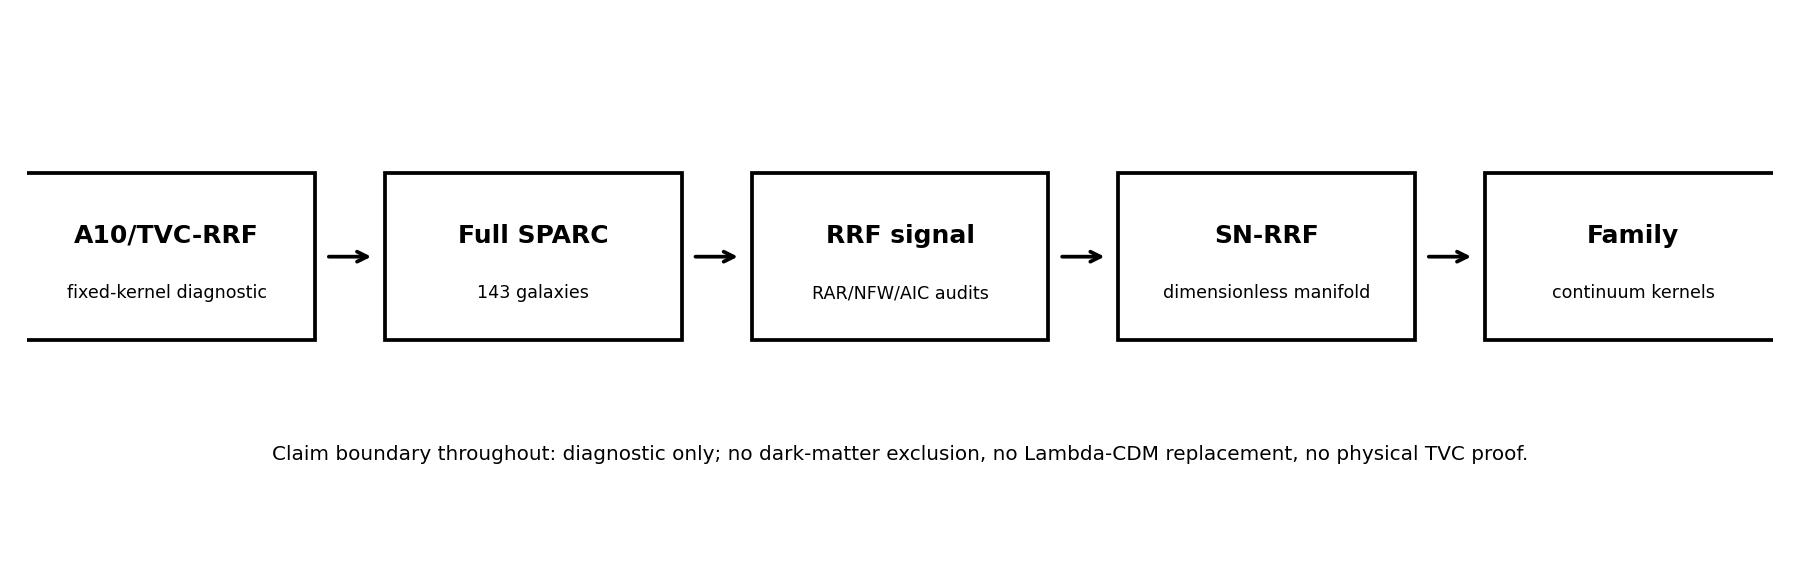
\includegraphics[width=0.96\linewidth]{../figures/integrated_audit_flow.png}
\caption{Integrated audit trajectory. The project begins with a fixed A10/TVC-RRF diagnostic kernel, tests it on the full eligible SPARC population, reformulates the surviving signal in dimensionless SN-RRF variables, and ends with a kernel-family rather than fixed-exponent synthesis. The claim boundary remains diagnostic-only throughout.}
\end{figure}

\begin{table}[H]
\centering
\caption{Condensed stage trajectory. ``Authorize'' means the next guarded diagnostic stage is justified; it does not mean physical promotion.}
\small
\begin{tabularx}{\linewidth}{>{\raggedright\arraybackslash}p{0.12\linewidth}X>{\raggedright\arraybackslash}p{0.25\linewidth}}
\toprule
Stage & Role & Locked interpretation \\
\midrule
Stage 7--10 & Full SPARC census, representative residual panels, evidence synthesis & A10/TVC-RRF survives as diagnostic residual-response framework only. \\
Stage 13R--16 & Population relation, RAR-relative comparison, stratification, adversarial guards & RRF amplitude has structured population relation; first-pass adversarial controls pass. \\
Stage 20--23 & Dimensionless SN-RRF band/manifold and stability audit & Strict rectangle inconclusive; central manifold plus pathology moat supported. \\
Stage 26 & Curve-level null-refit controls & Destructive nulls beaten; neighboring monotone kernels compete. \\
Stage 28--31 & Kernel-family and continuum-profile synthesis & Fixed-exponent uniqueness rejected; monotone-saturating response family supported. \\
\bottomrule
\end{tabularx}
\end{table}

\section{A10/TVC-RRF Full-Population Diagnostic Results}
The full eligible population contains 143 SPARC galaxies. In the broad-free full-population audit, A10/TVC-RRF shows strong improvement relative to baryonic-fit and remains competitive against comparator families. The final diagnostic synthesis carries forward the following central results.

\begin{table}[H]
\centering
\caption{Primary A10/TVC-RRF diagnostic results carried into the integrated paper. Negative $\dAIC$ values favor A10/TVC-RRF relative to the named comparator within the tested protocol.}
\small
\begin{tabularx}{\linewidth}{>{\raggedright\arraybackslash}p{0.38\linewidth}X}
\toprule
Audit item & Locked result \\
\midrule
Valid population count & 143 galaxies \\
Baryonic-fit comparison & median $\dAIC(\mathrm{TVC\mbox{-}RRF}-\mathrm{baryonic})=-475.791$ in full-census broad-free audit \\
RAR-relative comparison & median $\dAIC(\mathrm{TVC\mbox{-}RRF}-\mathrm{RAR\mbox{-}like})=-33.482$ \\
RAR-relative fractions & beats-RAR fraction = 0.867; strong beats-RAR fraction at $\dAIC\leq -10$ = 0.713; within +10 AIC fraction = 0.972 \\
Nuisance risk & Stage 14 nuisance-boundary rate = 0.217; maximum stratified nuisance-boundary rate = 0.417 \\
Population relation & $\mathrm{rrf\_log10\_A}$ vs $v_{\max}$: Spearman $\rho=0.873$; permutation $p=0.001996$ \\
Adversarial controls & 5/5 first-pass null-kernel and shuffled-label guards passed \\
\bottomrule
\end{tabularx}
\end{table}

The population relation is particularly important. It indicates that the fitted RRF amplitude is not merely an arbitrary per-galaxy curve-fitting knob; it is strongly associated with a basic rotation-curve scale. This is still not a physical-mechanism proof.

\section{Representative Residual Panels}
The following fixed-position panels summarize the Stage 9 representative residual-panel audit. They are not cherry-picked success examples: robust, nuisance-sensitive, NFW-dominant, weak/regime-dependent, and core-pathology cases are all included.

\begin{figure}[H]
\centering
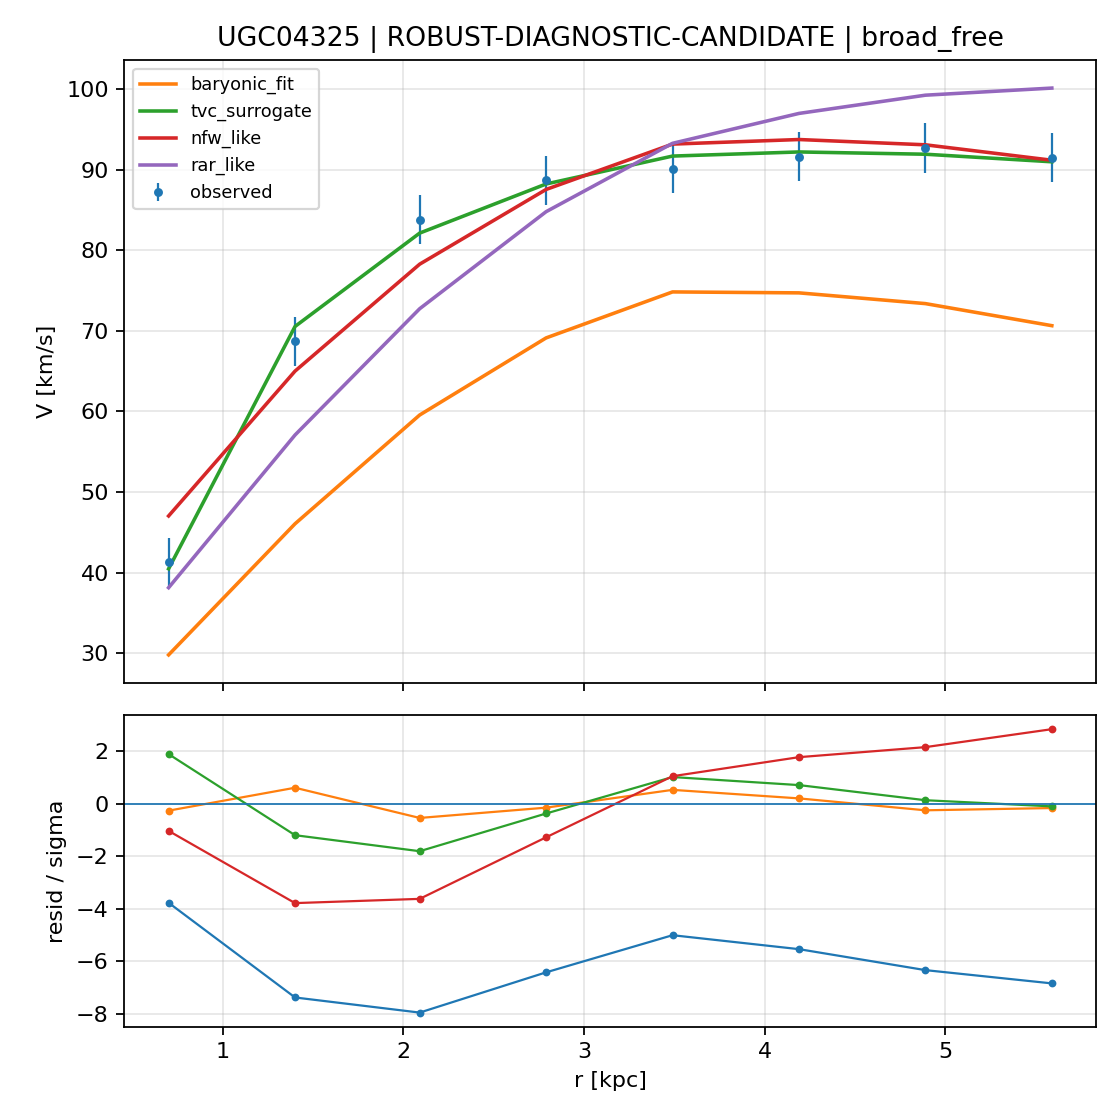
\includegraphics[width=0.32\linewidth]{../figures/fig1a_UGC04325.png}\hfill
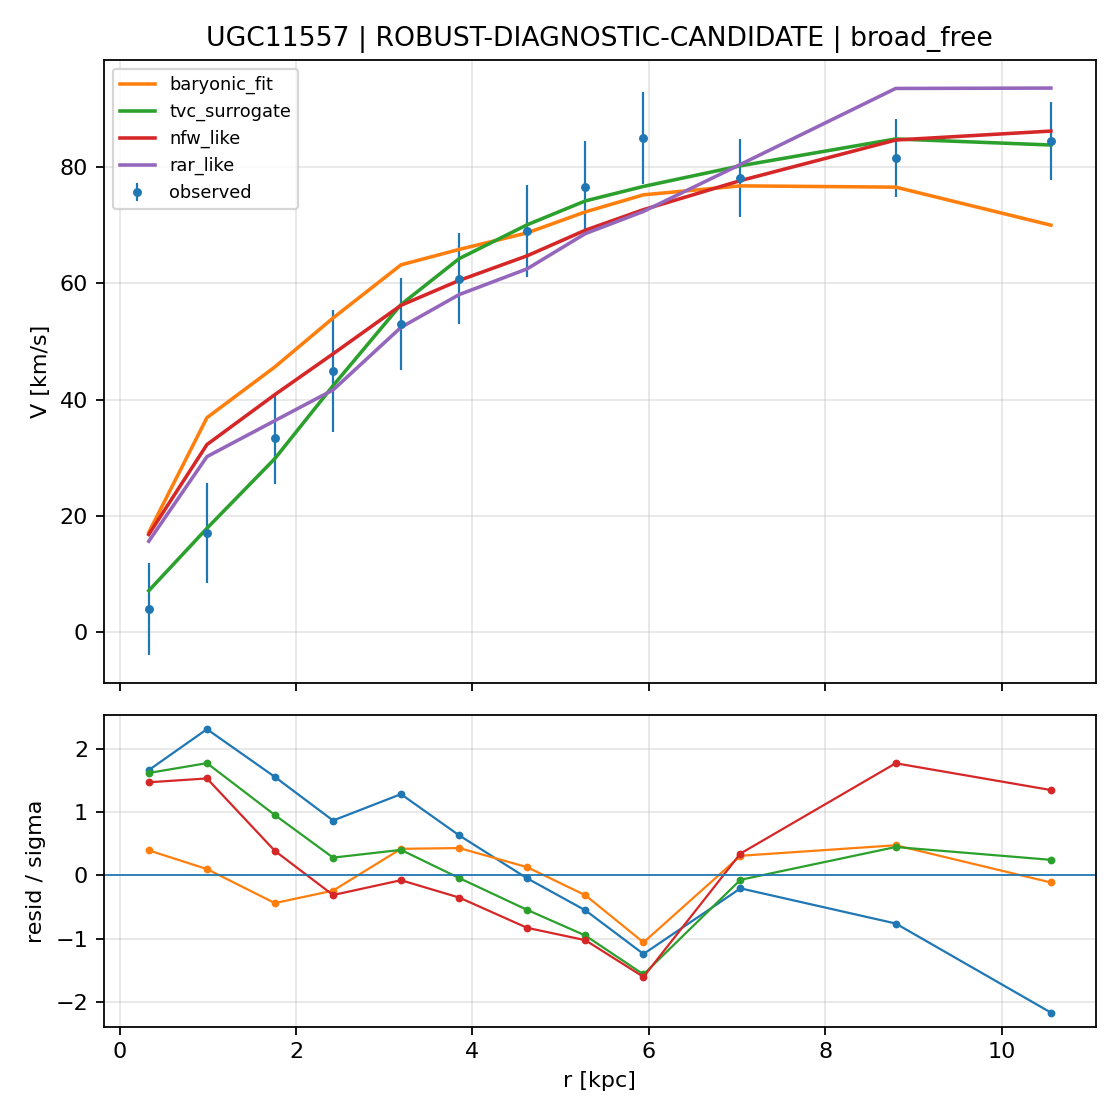
\includegraphics[width=0.32\linewidth]{../figures/fig1b_UGC11557.png}\hfill
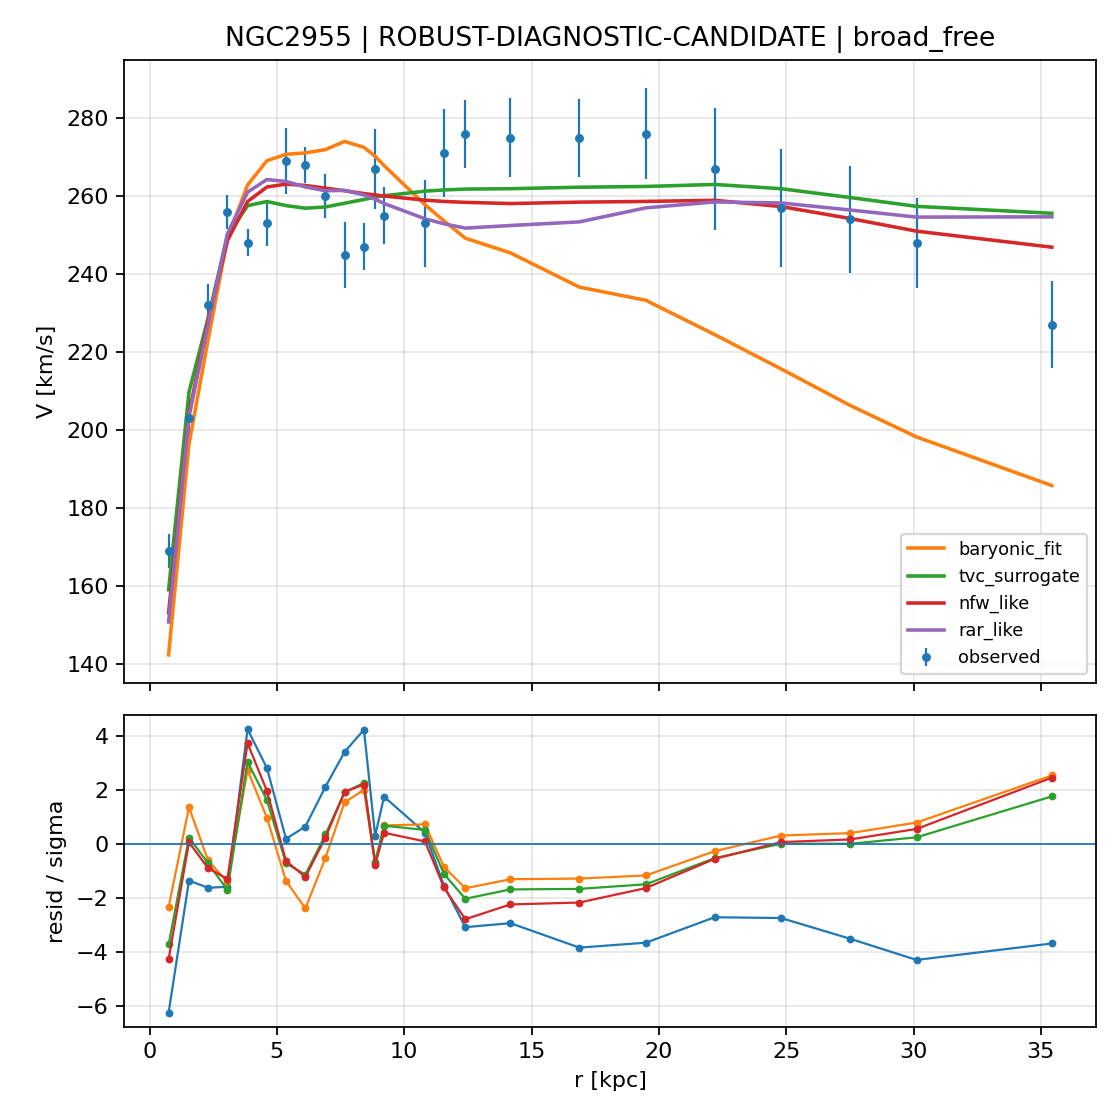
\includegraphics[width=0.32\linewidth]{../figures/fig1c_NGC2955.png}
\caption{Robust diagnostic candidates. These examples show cases where A10/TVC-RRF remains diagnostically competitive without recorded TVC boundary flags in the broad-free audit class. Panels: UGC04325, UGC11557, NGC2955.}
\end{figure}

\begin{figure}[H]
\centering
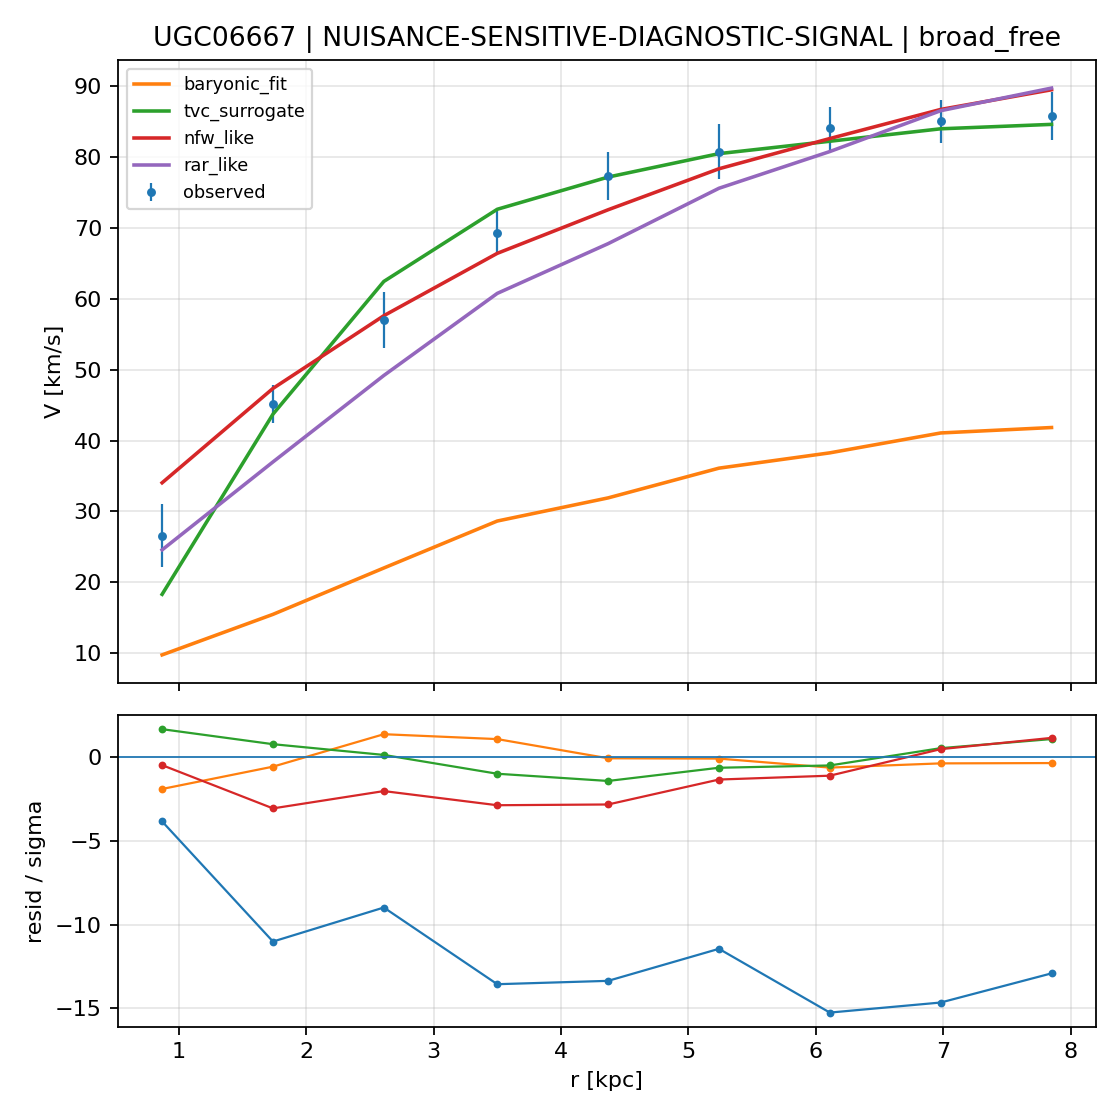
\includegraphics[width=0.32\linewidth]{../figures/fig2a_UGC06667.png}\hfill
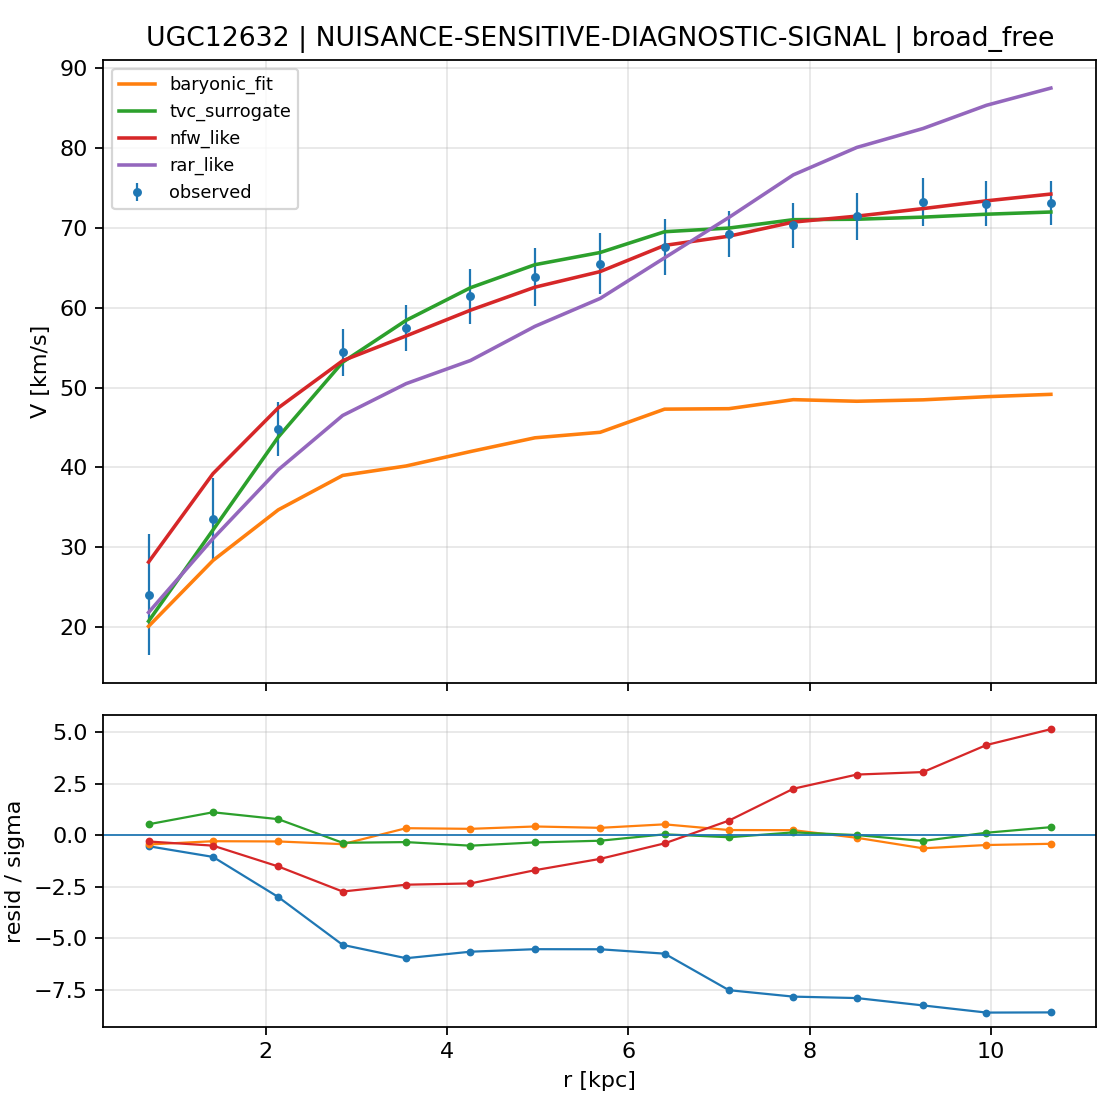
\includegraphics[width=0.32\linewidth]{../figures/fig2b_UGC12632.png}\hfill
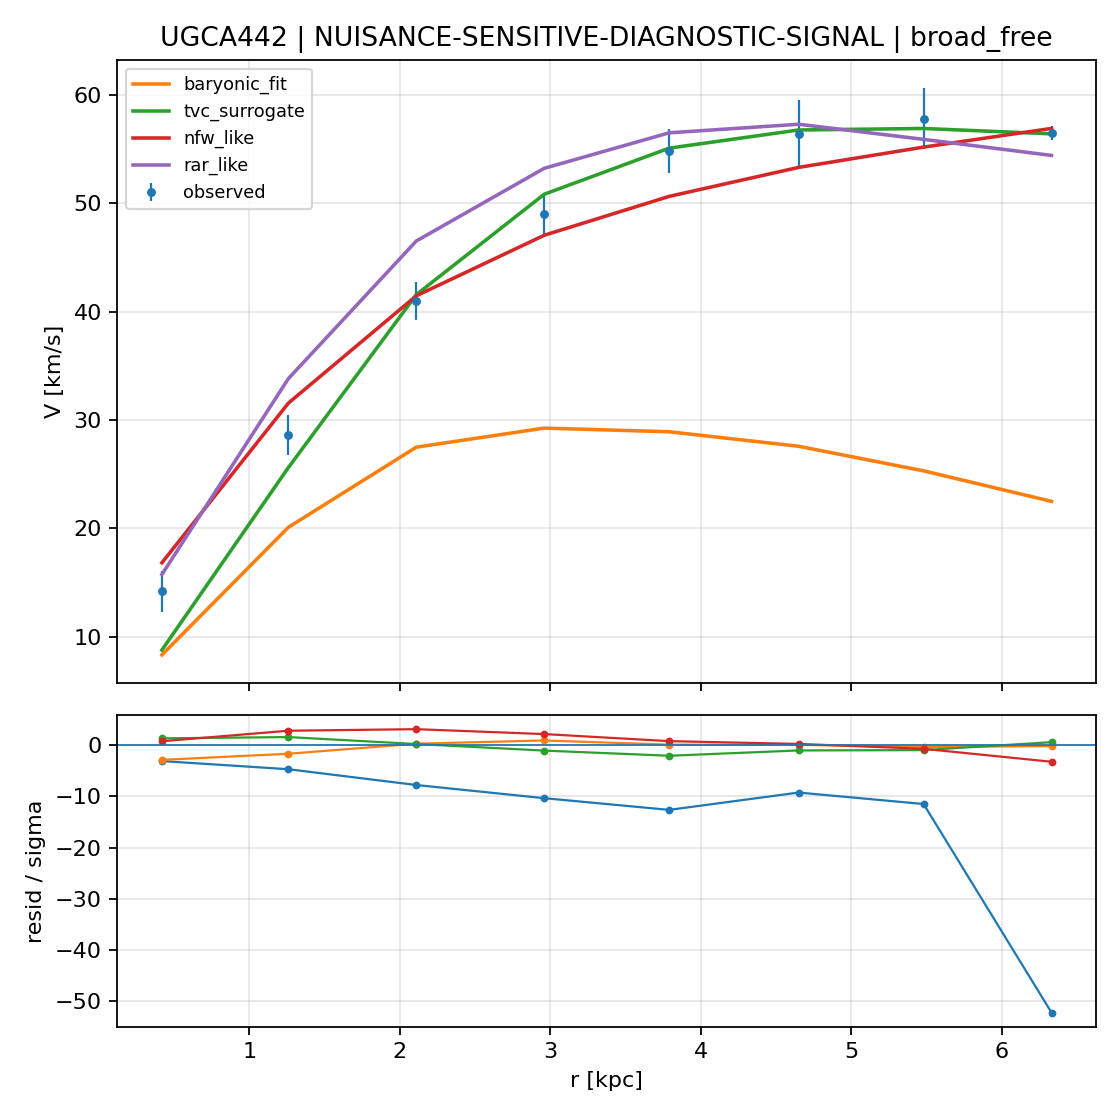
\includegraphics[width=0.32\linewidth]{../figures/fig2c_UGCA442.png}
\caption{Nuisance-sensitive diagnostic signals. These examples preserve diagnostic signal but require explicit reporting of stellar mass-to-light nuisance sensitivity. Panels: UGC06667, UGC12632, UGCA442.}
\end{figure}

\begin{figure}[H]
\centering
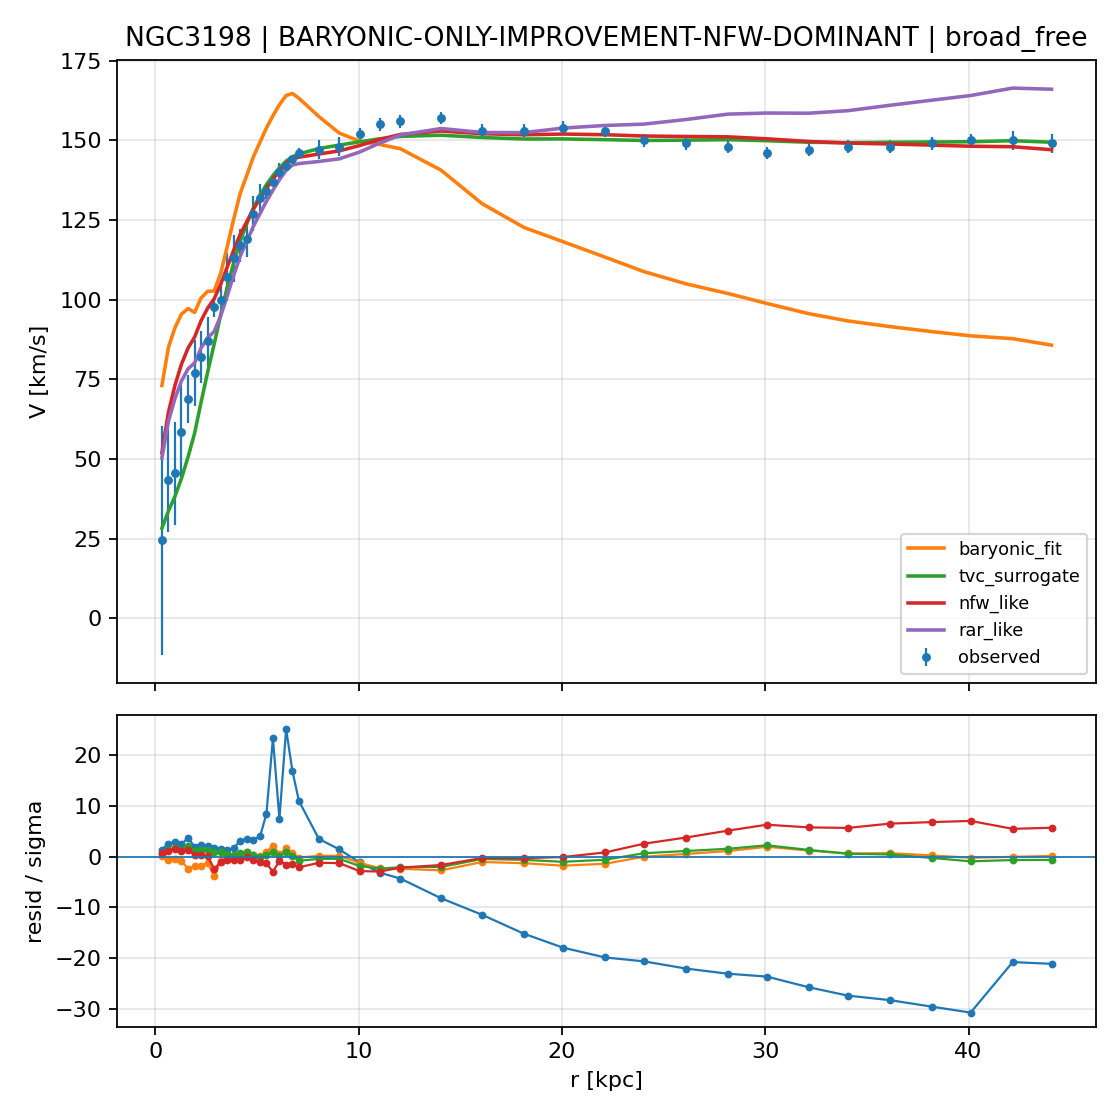
\includegraphics[width=0.32\linewidth]{../figures/fig3a_NGC3198.png}\hfill
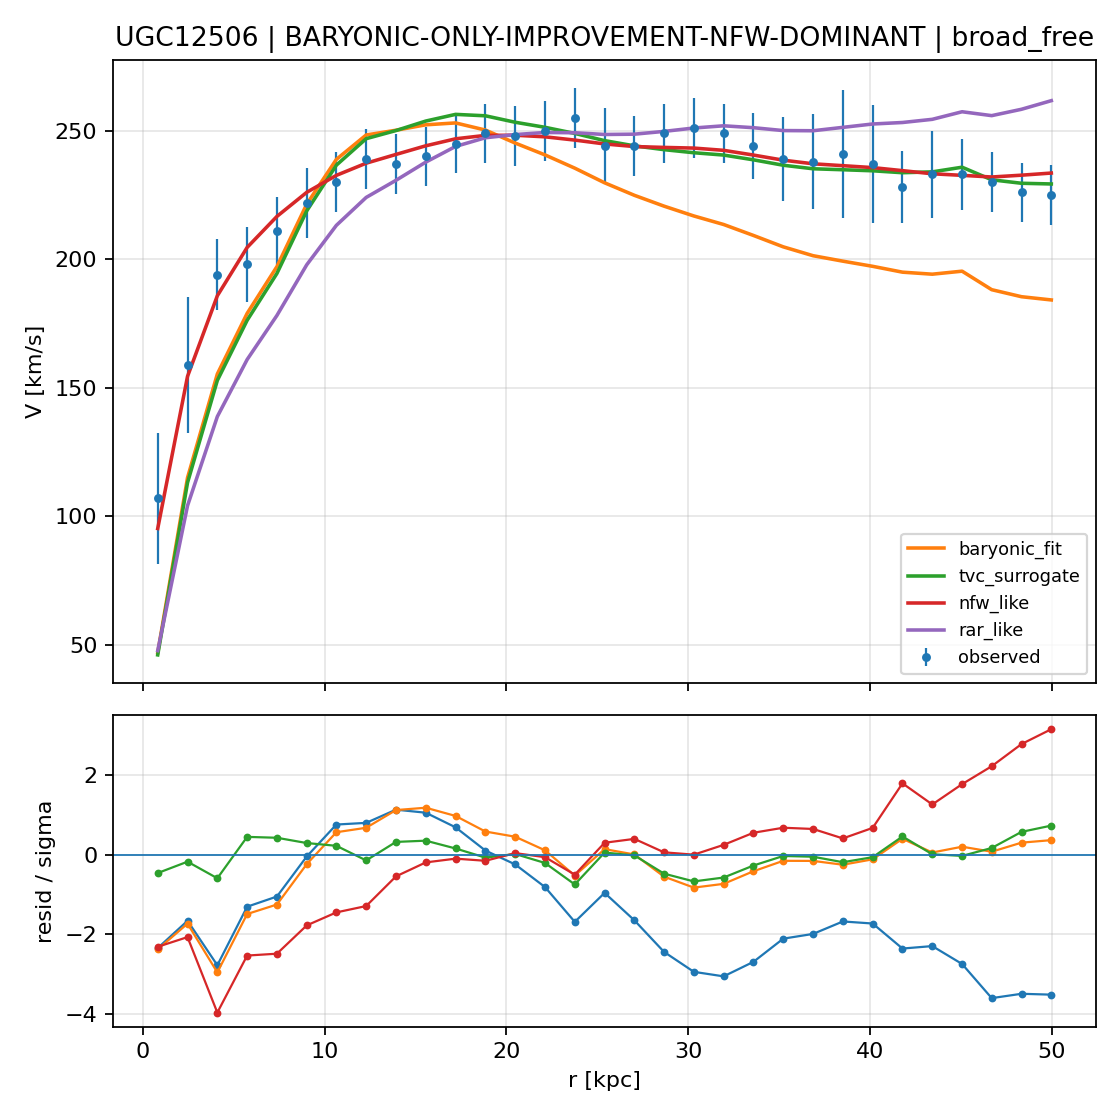
\includegraphics[width=0.32\linewidth]{../figures/fig3b_UGC12506.png}\hfill
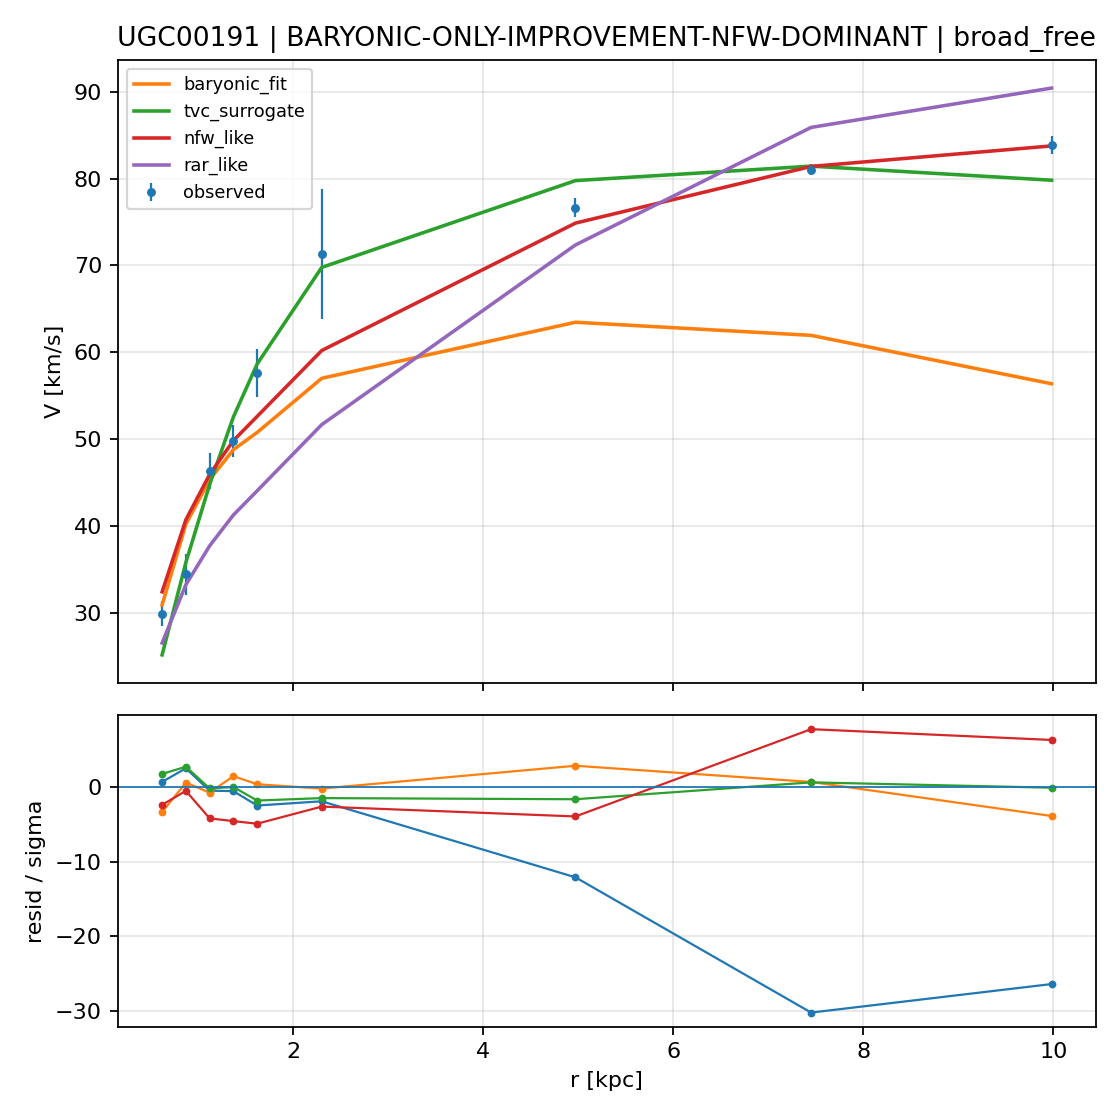
\includegraphics[width=0.32\linewidth]{../figures/fig3c_UGC00191.png}
\caption{Baryonic-only improvement but NFW-dominant cases. These examples improve over the baryonic-fit baseline but remain less favorable than the NFW-like comparator. Panels: NGC3198, UGC12506, UGC00191.}
\end{figure}

\begin{figure}[H]
\centering
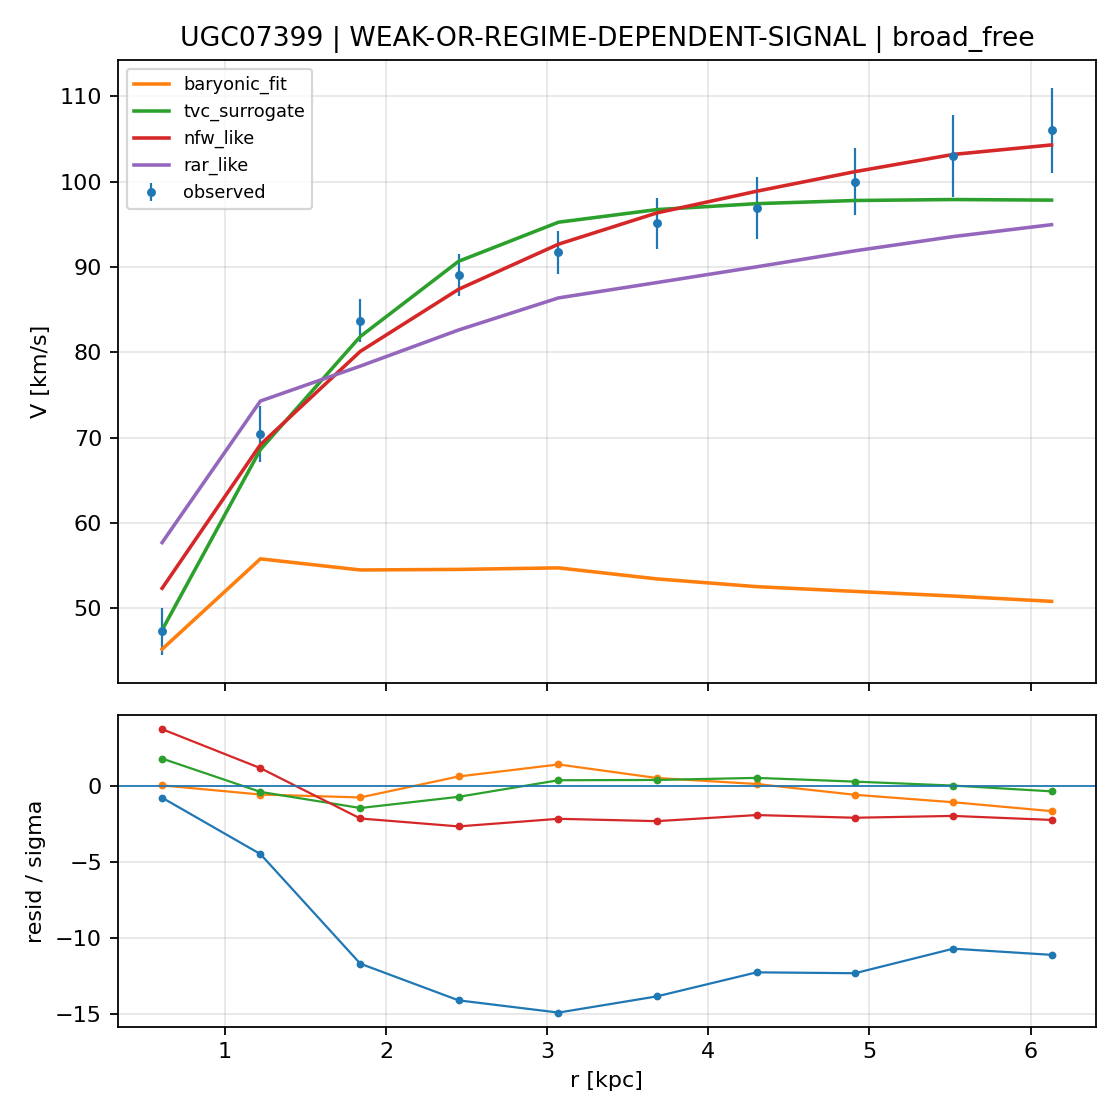
\includegraphics[width=0.32\linewidth]{../figures/fig4a_UGC07399.png}\hfill
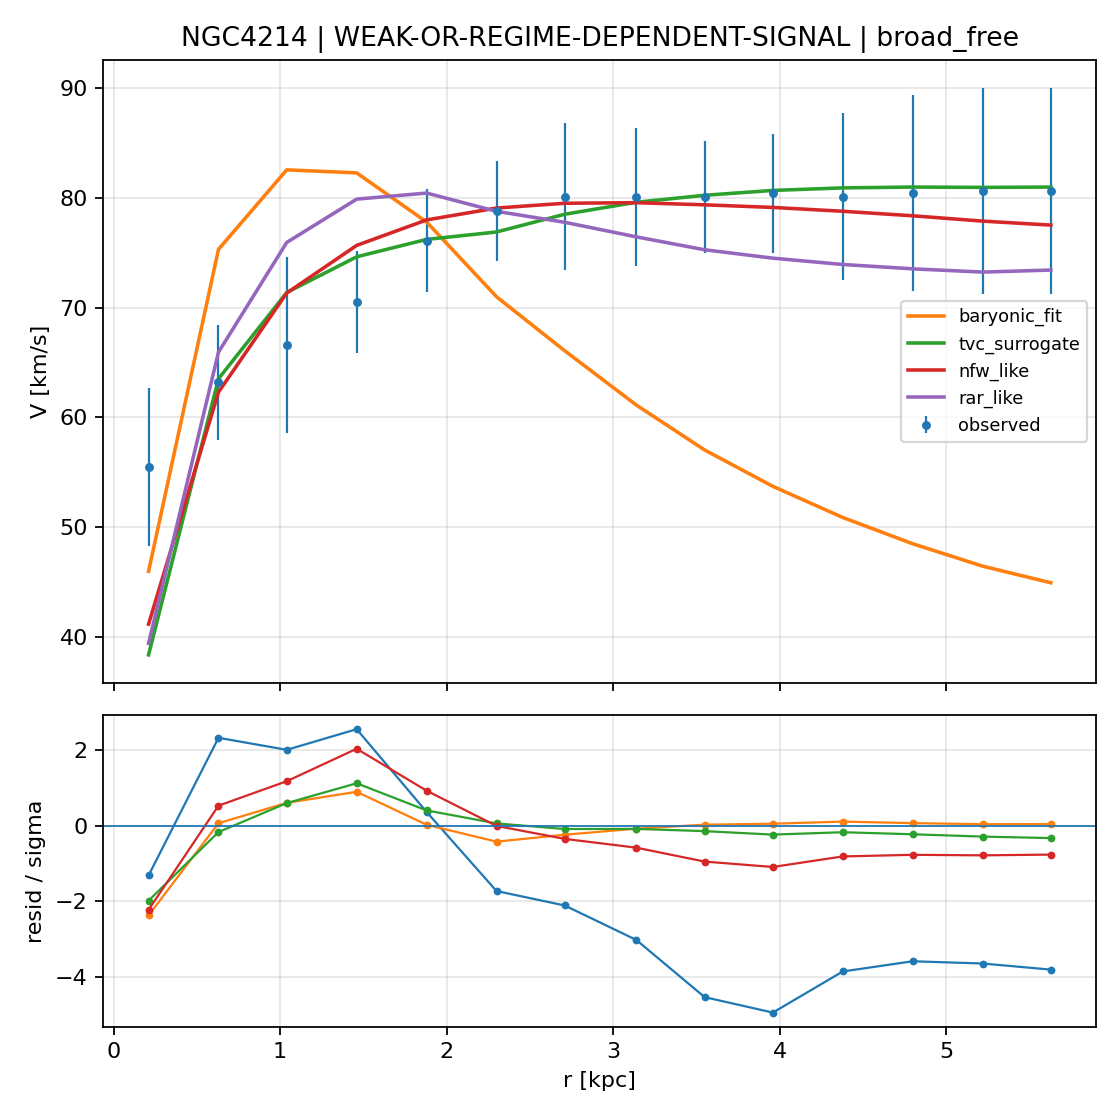
\includegraphics[width=0.32\linewidth]{../figures/fig4b_NGC4214.png}\hfill
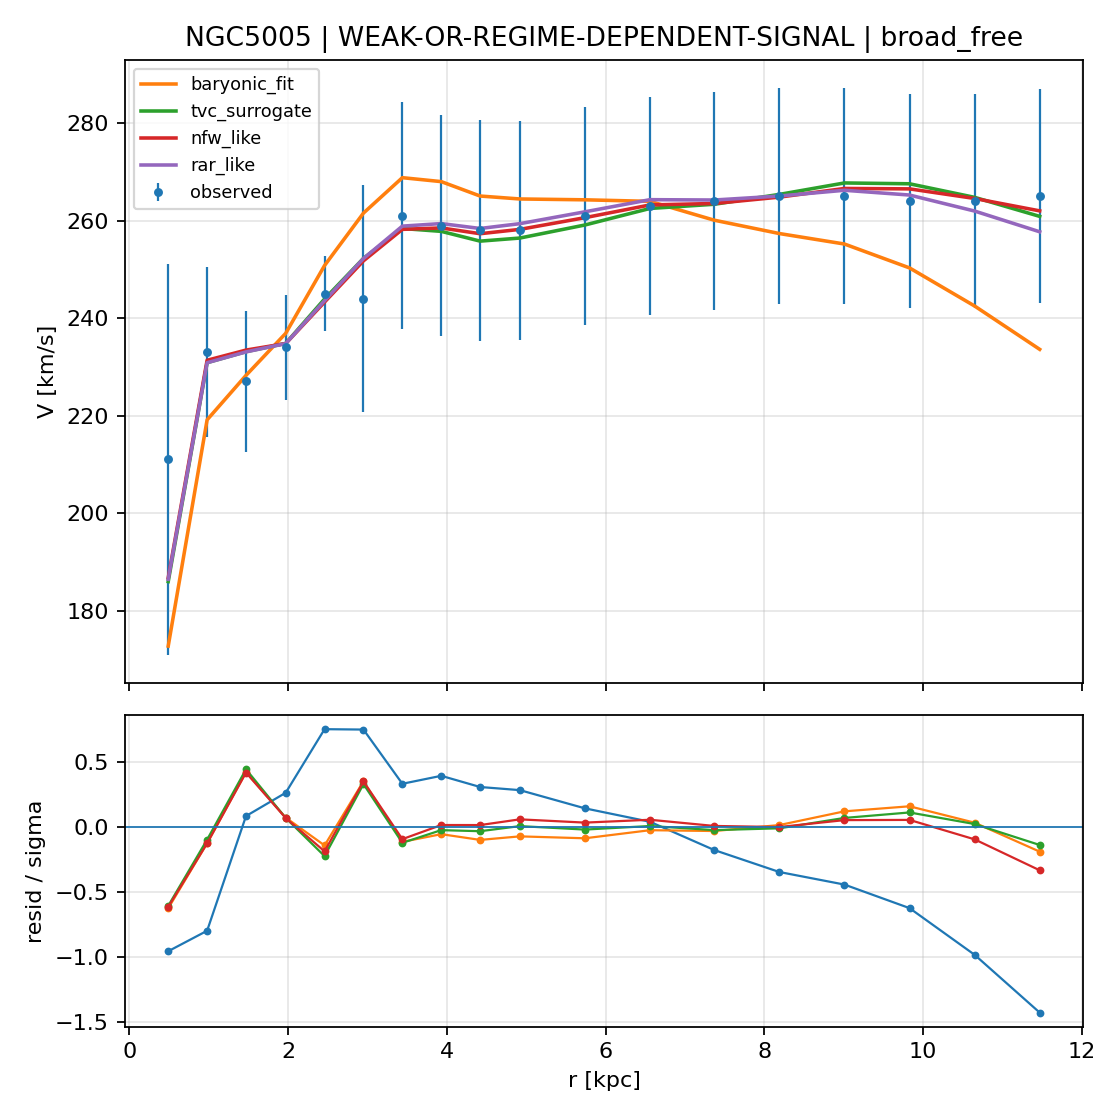
\includegraphics[width=0.32\linewidth]{../figures/fig4c_NGC5005.png}
\caption{Weak or regime-dependent cases. These examples illustrate cases where the diagnostic signal is present but not robustly dominant across comparison regimes. Panels: UGC07399, NGC4214, NGC5005.}
\end{figure}

\begin{figure}[H]
\centering
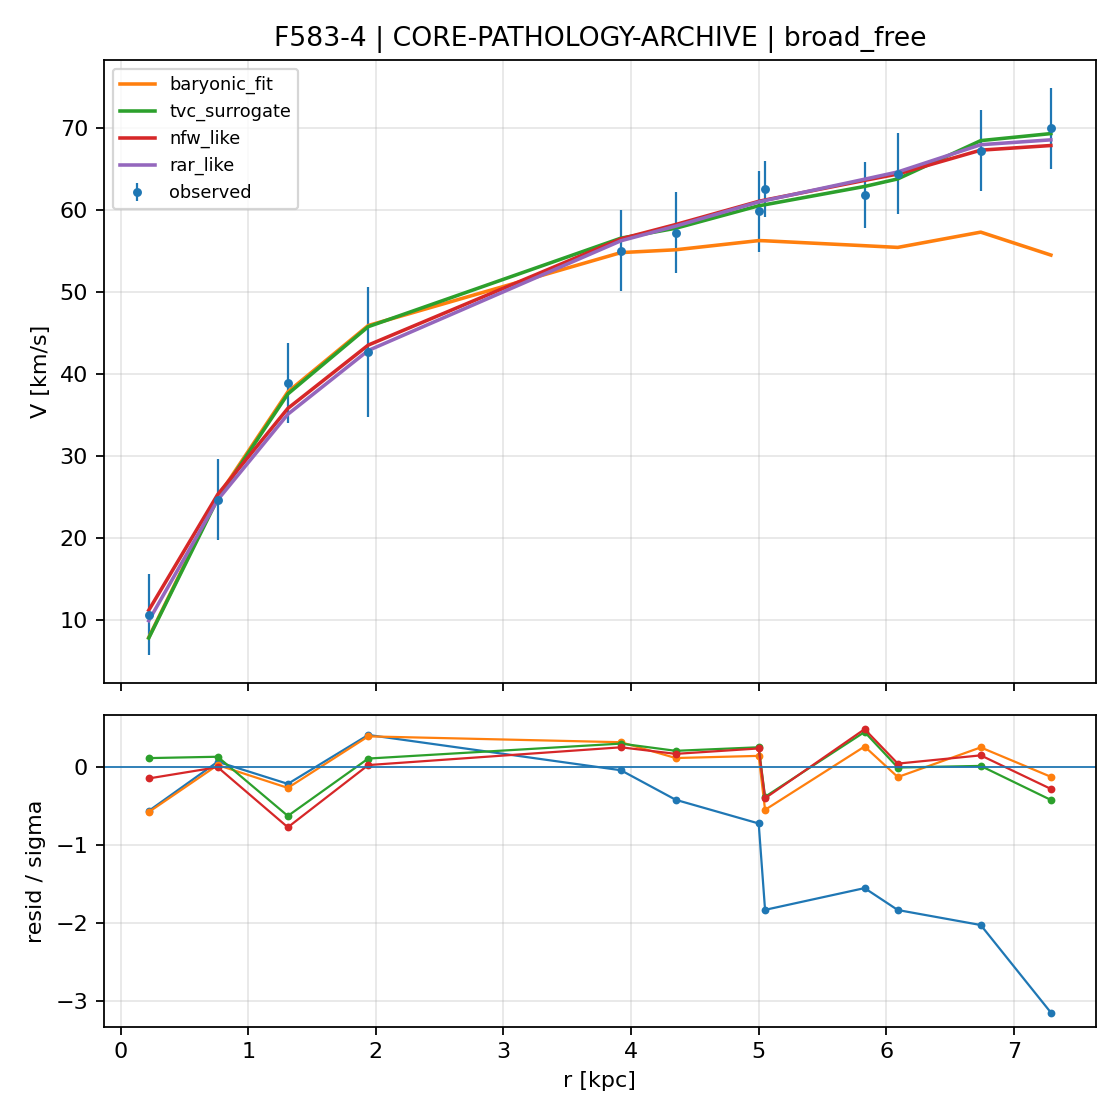
\includegraphics[width=0.32\linewidth]{../figures/fig5a_F583-4.png}\hfill
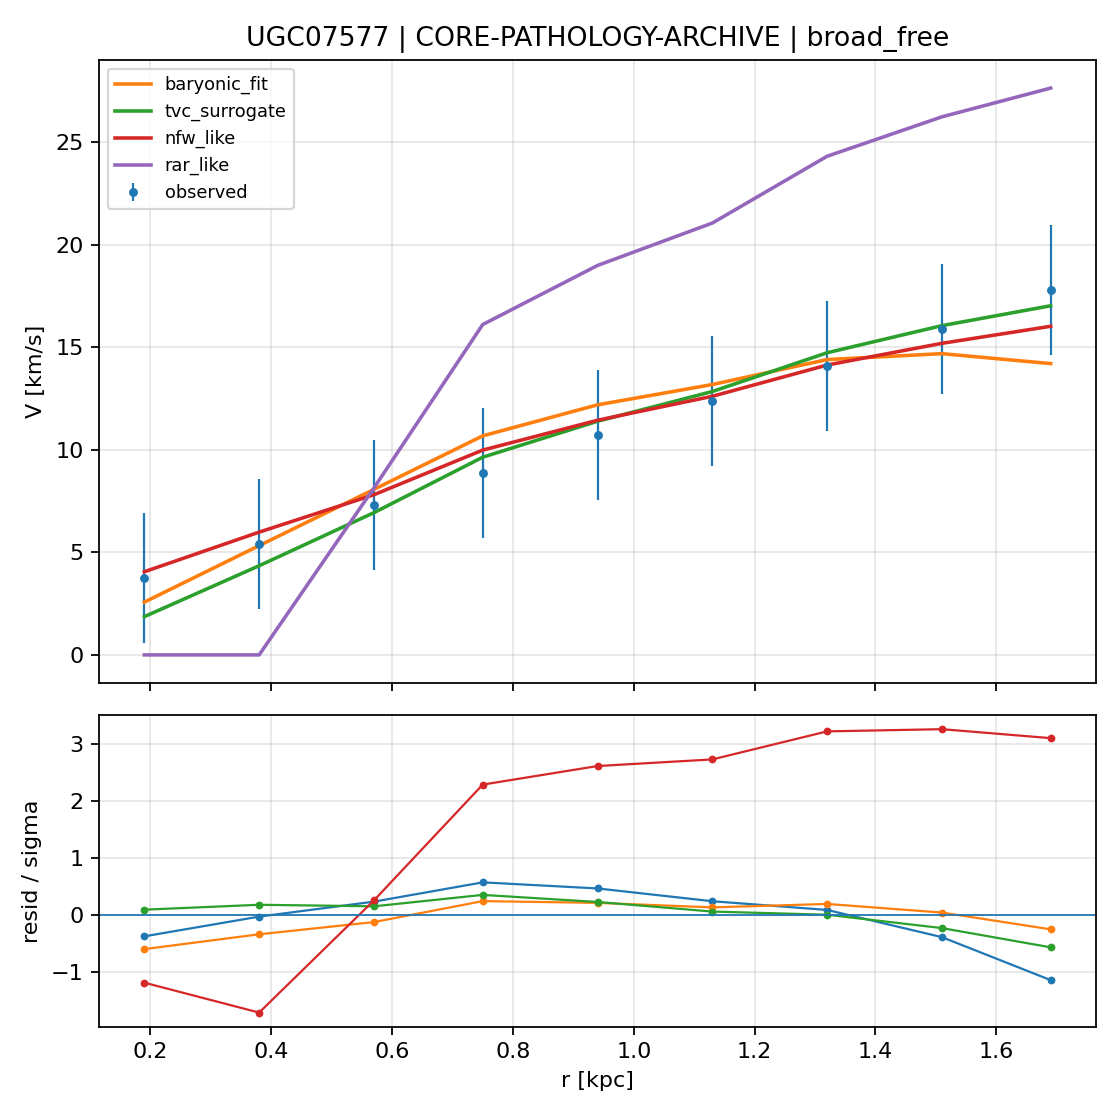
\includegraphics[width=0.32\linewidth]{../figures/fig5b_UGC07577.png}\hfill
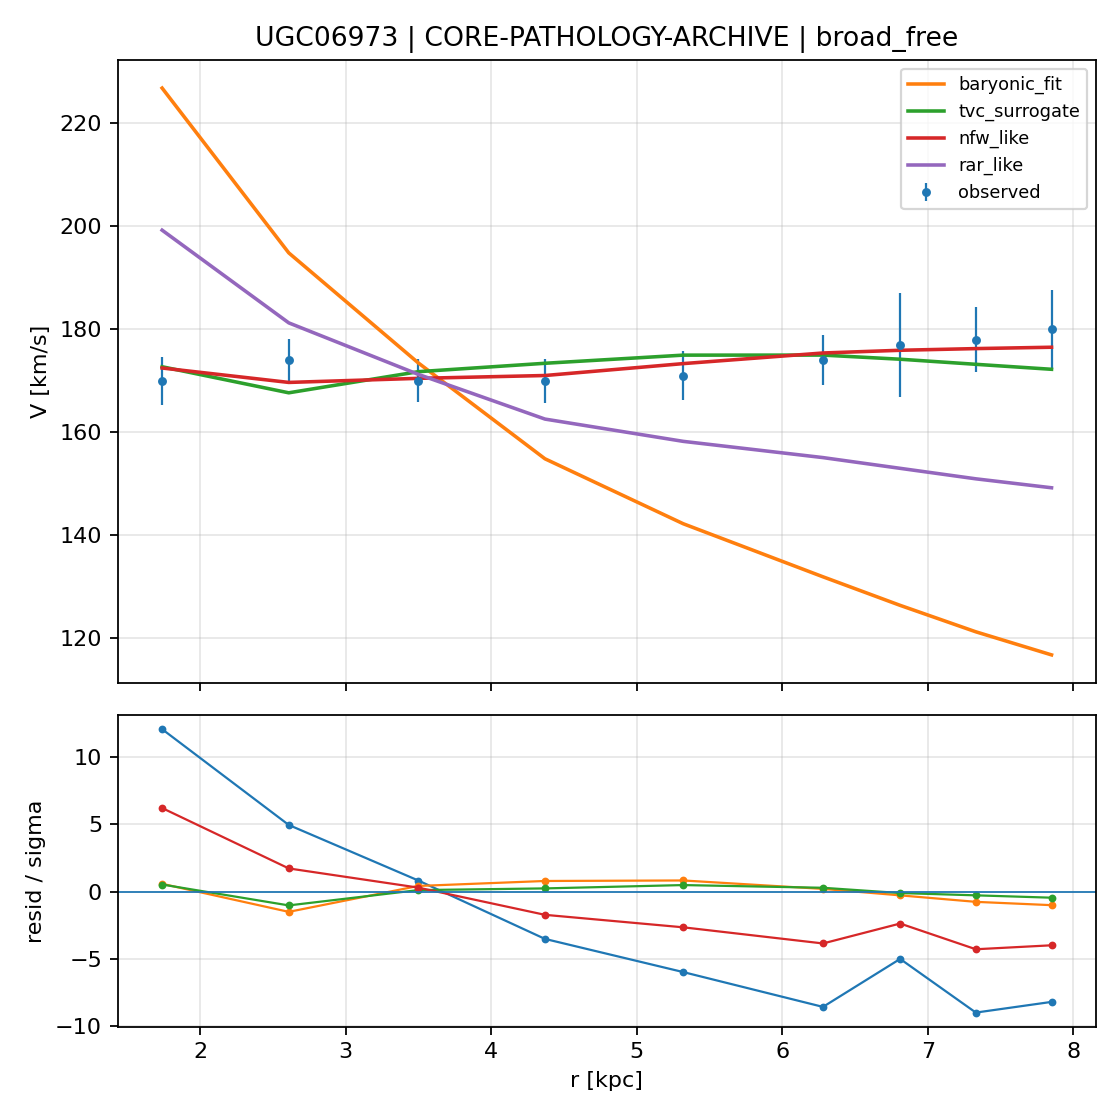
\includegraphics[width=0.32\linewidth]{../figures/fig5c_UGC06973.png}
\caption{Core-pathology archive cases. These examples are included as negative controls and are not promoted as successful A10/TVC-RRF cases. Panels: F583-4, UGC07577, UGC06973.}
\end{figure}

\section{Beyond A10/TVC: Dimensionless SN-RRF Manifold}
Stage 20 tested whether a strict rectangular normal-response band could describe individual galaxies. The result was inconclusive: all-normal-band fraction = 0.490 and robust-in-normal-band fraction = 0.481, although pathology-class in pathology band fraction = 0.857. Therefore, the strict rectangle is not promoted as a universal per-galaxy law.

Stage 21 repaired the claim to a weaker, more defensible manifold statement. Non-pathology class medians remain inside the proposed dimensionless response neighborhood, the pathology-class median lies inside the pathology moat, the nonpathology false-positive rate is 0.000, and the pathology moat hit rate is 0.857. A robust-candidate-calibrated q90 manifold includes 0.896 of robust candidates and 0.860 of nonpathology cases while excluding 0.857 of pathology cases.

\begin{figure}[H]
\centering
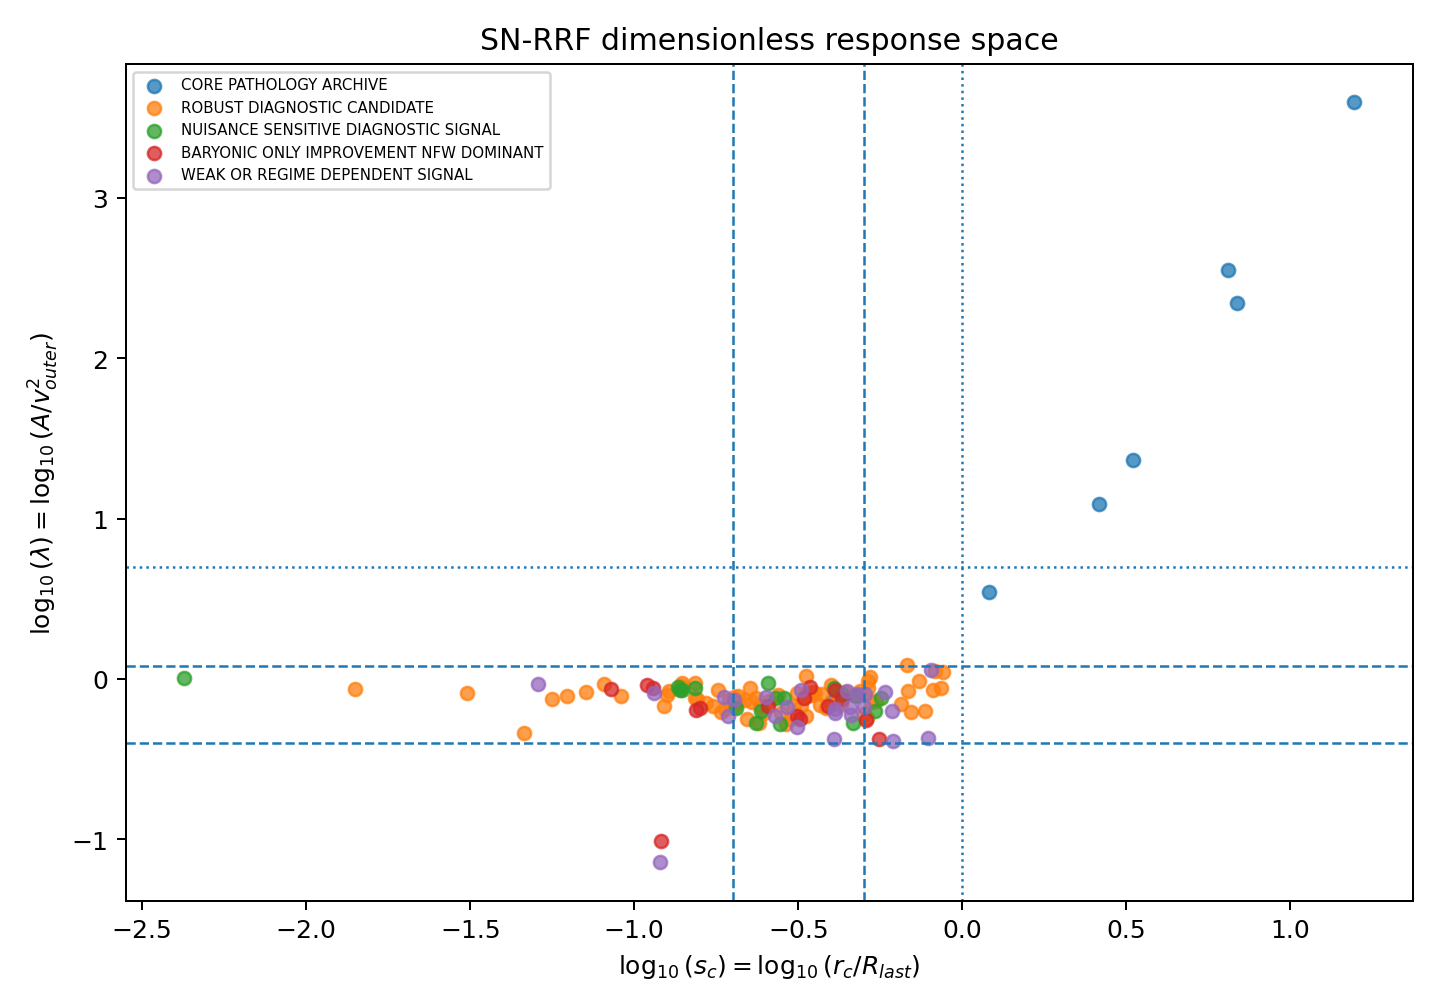
\includegraphics[width=0.86\linewidth]{../figures/stage21_manifold_scatter.png}
\caption{SN-RRF dimensionless response space. The variables are $\log_{10}(\scc)$ and $\log_{10}(\lam)$. Dashed reference lines indicate the originally proposed normal-response rectangle; dotted reference lines mark the pathology-moat thresholds. The figure illustrates why a strict rectangle is too strong, while a central-manifold plus pathology-separation interpretation is more defensible.}
\end{figure}

Stage 23 stress-tests this interpretation by bootstrap recalibration and shuffled-label/permutation controls. The result is 7/7 guard pass. The pathology-minus-nonpathology median distance separation is 18.450 with one-sided permutation $p=0.00049975$. Bootstrap medians are robust-inside fraction = 0.896, nonpath-inside fraction = 0.853, and pathology-exclusion fraction = 0.857.

\begin{table}[H]
\centering
\caption{SN-RRF dimensionless manifold and stability results.}
\small
\begin{tabularx}{\linewidth}{>{\raggedright\arraybackslash}p{0.45\linewidth}X}
\toprule
Metric & Result \\
\midrule
Stage 20 strict band decision & weak hold; rectangular normal band inconclusive \\
All normal-band fraction & 0.490 \\
Robust normal-band fraction & 0.481 \\
Pathology class in pathology band & 0.857 \\
Stage 21 nonpathology false-positive rate into pathology moat & 0.000 \\
Stage 21 robust q90 manifold inside fraction & 0.896 \\
Stage 21 nonpathology q90 manifold inside fraction & 0.860 \\
Stage 21 pathology q90 manifold exclusion fraction & 0.857 \\
Stage 23 guard result & 7/7 guards passed \\
Stage 23 permutation separation test & one-sided $p=0.00049975$ \\
\bottomrule
\end{tabularx}
\end{table}

\section{Curve-Level Null-Refit Controls}
Stage 26 refits curve-level squared-velocity residuals directly against the locked SN-RRF/A10-TVC-RRF kernel and adversarial null kernels. This is diagnostic only and does not reproduce the earlier nonlinear velocity-space audit exactly. The destructive nulls include constant floor, outer step median, reversed fixed RRF, and shuffled-radius fixed RRF. Neighbor monotone kernels include arctan, exponential, and saturating $n=1,2,4,6,8$ forms.

\begin{figure}[H]
\centering
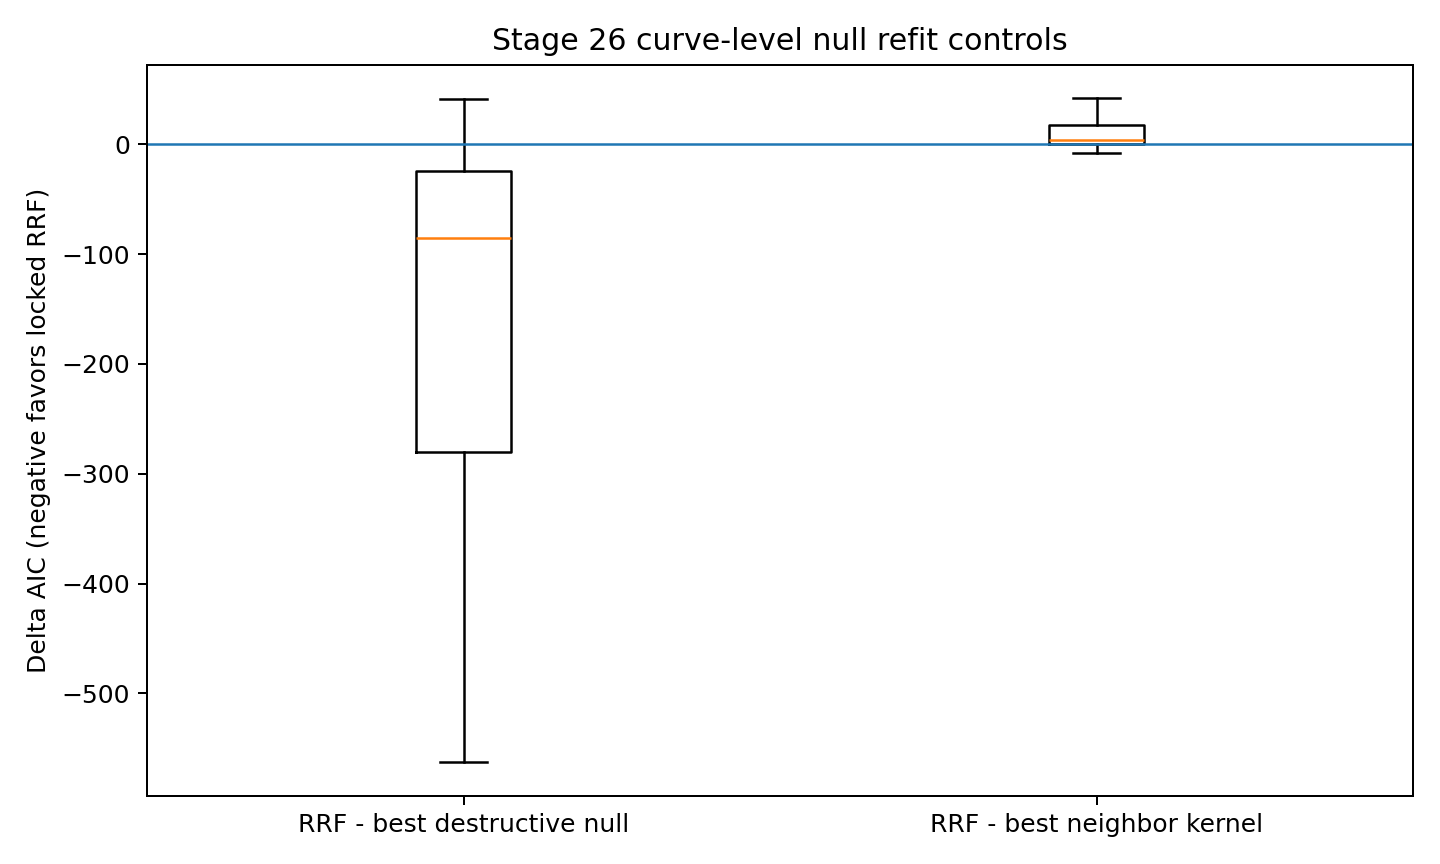
\includegraphics[width=0.82\linewidth]{../figures/stage26_null_refit_boxplot.png}
\caption{Stage 26 curve-level null-refit controls. Negative $\dAIC$ favors the locked RRF. The locked kernel strongly beats destructive nulls, but neighboring monotone-saturating kernels compete. This supports radial-response family structure, not fixed-exponent uniqueness.}
\end{figure}

The locked kernel beats the best destructive null in 0.916 of galaxies, strongly beats it at $\dAIC\leq -10$ in 0.839, and does so in 0.935 of robust-class galaxies. However, relative to the best neighbor monotone kernel, median $\dAIC(\mathrm{locked}-\mathrm{best\ neighbor})=4.082$ and the locked kernel wins in only 0.126 of galaxies. The correct synthesis is not that $n=3.258993$ is unique, but that a monotone-saturating response family is present.

\section{Kernel-Family and Continuum Synthesis}
Stage 28 profiles the monotone-saturating kernel family after Stage 26. Per-galaxy best-neighbor counts are led by saturating $n=2$ with 67/143 galaxies, followed by saturating $n=4$ with 26/143, saturating $n=1$ with 16/143, saturating $n=8$ with 12/143, arctan with 10/143, exponential with 8/143, and saturating $n=6$ with 4/143. A full per-kernel table is available, and the family-level interpretation is authorized.

Stage 30 then scans a 41-point continuum grid over
\begin{equation}
K_n(x)=\frac{x^n}{1+x^n}, \qquad n\in[0.5,12.0].
\end{equation}
The best exponent is heterogeneous: best-$n$ median = 2.25, IQR = [1.5, 3.2545]. The locked exponent is within +2 AIC of the continuum best in 0.322 of galaxies and within +10 AIC in 0.636. The continuum audit passes 6/6 guards.

\begin{figure}[H]
\centering
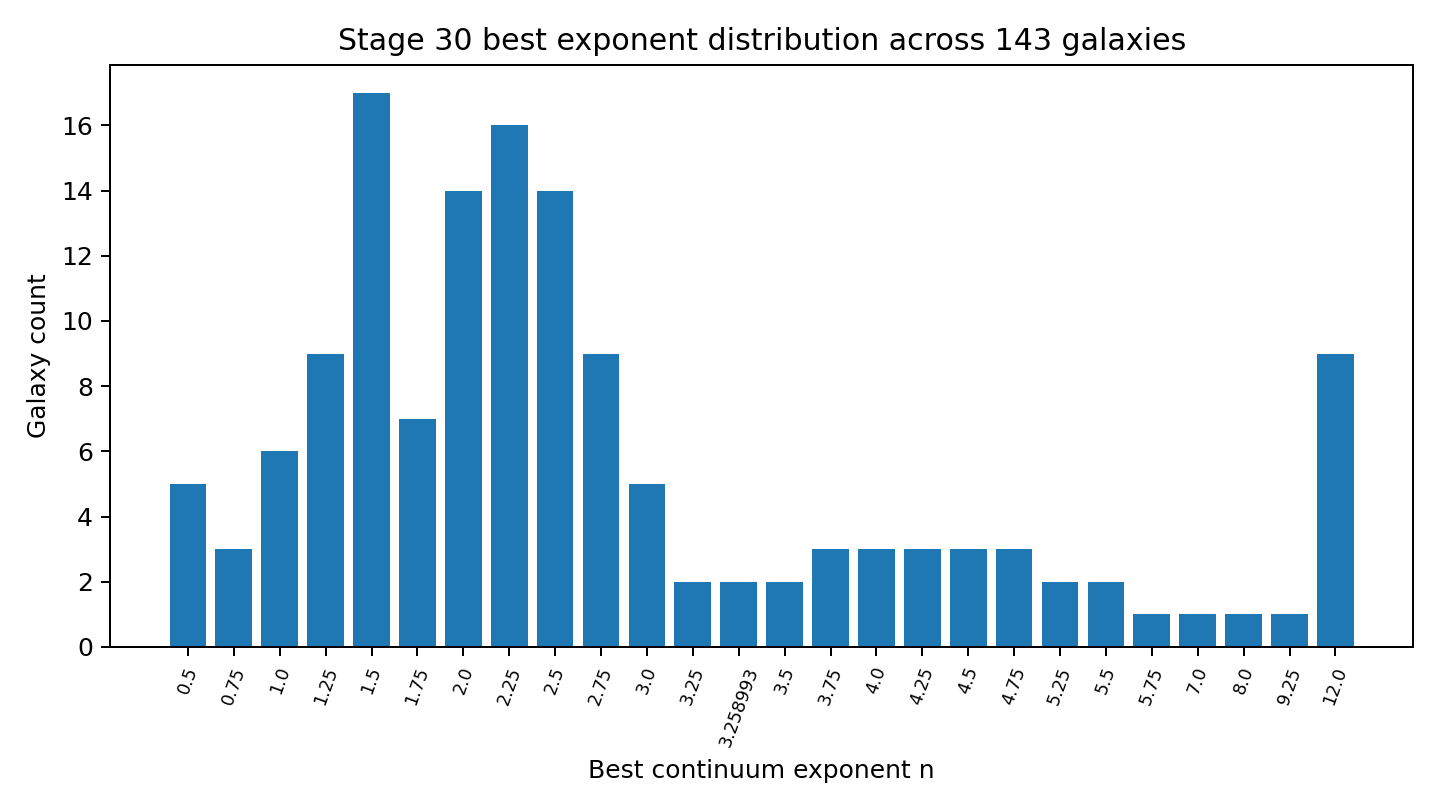
\includegraphics[width=0.88\linewidth]{../figures/stage30_best_n_distribution.png}
\caption{Stage 30 best-$n$ distribution. The best continuum exponent varies across galaxies, which rejects fixed-exponent uniqueness and supports a heterogeneous monotone-saturating residual-response family.}
\end{figure}

\begin{table}[H]
\centering
\caption{Kernel-family and continuum-profile synthesis.}
\small
\begin{tabularx}{\linewidth}{>{\raggedright\arraybackslash}p{0.45\linewidth}X}
\toprule
Metric & Result \\
\midrule
Stage 26 destructive-null guard result & 5/5 guards passed \\
RRF beats best destructive null fraction & 0.916 \\
RRF strongly beats best destructive null fraction & 0.839 \\
RRF beats best neighbor monotone kernel fraction & 0.126 \\
Stage 28 best-neighbor leader & saturating $n=2$ with 67/143 galaxies \\
Stage 30 continuum grid & 41 points, $n=0.5$ to $12.0$ \\
Best-$n$ median & 2.25 \\
Best-$n$ IQR & [1.5, 3.2545] \\
Locked $n$ within +2 AIC of continuum best & 0.322 \\
Locked $n$ within +10 AIC of continuum best & 0.636 \\
Stage 30 guard result & 6/6 guards passed \\
Final kernel interpretation & scale-normalized monotone-saturating residual-response family, not unique fixed exponent \\
\bottomrule
\end{tabularx}
\end{table}

\section{Integrated Interpretation}
The project began with a risky old framing: a fixed exponent near 3.26 was associated with broad cosmological and dark-matter claims. The integrated audit shows that those broad claims are not justified. However, it also shows that something nontrivial survives once the claim boundary is enforced.

The surviving structure is not a proof of a physical medium or modified-gravity mechanism. It is a residual-response family with three diagnostic properties:
\begin{enumerate}
  \item \textbf{A galaxy-scale residual signal}: A10/TVC-RRF improves over baryonic baselines and remains diagnostically competitive in RAR-relative audits under the tested protocol.
  \item \textbf{A population-scale relation}: RRF amplitude is strongly associated with maximum rotation velocity.
  \item \textbf{A dimensionless family structure}: after scale normalization, nonpathology cases cluster around a central manifold, pathology cases are separated by a moat, and the curve-level radial-response shape beats destructive nulls while belonging to a broader monotone-saturating kernel family.
\end{enumerate}

The practical meaning is limited but useful: the old fixed-exponent ansatz should not be treated as a new physical law, but the residual-response geometry it exposed is sufficiently structured to justify a narrower diagnostic vocabulary and further tests.

\section{Limitations and Future Work}
The strongest limitation is that all claims remain diagnostic. The model does not include a physical dark-matter halo interpretation, modified gravity derivation, cosmological perturbation treatment, or independent external validation. Stellar mass-to-light nuisance sensitivity remains a reported limitation in the A10/TVC-RRF audit. Stage 26 curve-level null-refit controls use fixed stellar mass-to-light values and squared-velocity residual fits, so they are an adversarial diagnostic control rather than a complete replacement for the earlier nonlinear fitting protocol.

A future version should test out-of-sample SPARC splits, alternative baryonic prescriptions, hierarchical Bayesian kernel-family fitting, explicit halo-comparison fairness controls, and external galaxy samples. If this residual-response methodology is later applied to cosmological expansion data, it must be tested separately on supernova, BAO, CMB, distance-ladder, and $H_0$ datasets. The present paper does not address the Hubble tension directly.

\section{Conclusion}
This integrated audit supports a conservative but nontrivial diagnostic conclusion within the tested protocol. A10/TVC-RRF survives as a fixed-kernel diagnostic representative, but fixed-exponent uniqueness does not survive. The better final synthesis is SN-RRF: a Scale-Normalized Residual Response Family for SPARC galaxy rotation-curve residuals.

SN-RRF is supported, within the tested protocol, as a diagnostic residual-response family and pathology-separation framework. It is not evidence for dark-matter exclusion, Lambda-CDM replacement, MOND/RAR defeat, a Bullet-Cluster explanation, a physical TVC mechanism, or a Hubble-tension solution.

\section*{Code and Reproducibility Availability}
The GitHub repository associated with this manuscript is available at \href{https://github.com/yokken0907/a10-tvc-rrf-galaxy-residual-diagnostic}{github.com/yokken0907/a10-tvc-rrf-galaxy-residual-diagnostic}. The repository package contains the manuscript sources, result summaries, figures, scripts, claim-boundary material, and browser-only project visual orientation files.

The Zenodo identifier \href{https://doi.org/10.5281/zenodo.20224479}{10.5281/zenodo.20224479} refers to an archived repository release, not to a separately peer-reviewed article DOI. If this reader-guidance revision is archived as a new GitHub/Zenodo release, the current version DOI should be cited as the companion repository-archive DOI for that release, while the prior DOI remains part of the repository history.

\section*{Acknowledgements}
The author used AI assistance, including OpenAI ChatGPT, for theory structuring, verification-protocol organization, code-drafting support, numerical-audit workflow organization, and manuscript editing support. The author reviewed the outputs and is responsible for the final scientific claims, claim boundaries, interpretation, and manuscript content.

\begin{thebibliography}{99}
\bibitem{Akaike1974AIC}
Akaike, H. (1974). A new look at the statistical model identification. \emph{IEEE Transactions on Automatic Control}. DOI: \href{https://doi.org/10.1109/TAC.1974.1100705}{10.1109/TAC.1974.1100705}.

\bibitem{Lelli2016SPARC}
Lelli, F., McGaugh, S. S., and Schombert, J. M. (2016). SPARC: Mass Models for 175 Disk Galaxies with Spitzer Photometry and Accurate Rotation Curves. \emph{The Astronomical Journal}. DOI: \href{https://doi.org/10.3847/0004-6256/152/6/157}{10.3847/0004-6256/152/6/157}.

\bibitem{McGaugh2016RAR}
McGaugh, S. S., Lelli, F., and Schombert, J. M. (2016). Radial Acceleration Relation in Rotationally Supported Galaxies. \emph{Physical Review Letters}. DOI: \href{https://doi.org/10.1103/PhysRevLett.117.201101}{10.1103/PhysRevLett.117.201101}.

\bibitem{Milgrom1983MOND}
Milgrom, M. (1983). A modification of the Newtonian dynamics as a possible alternative to the hidden mass hypothesis. \emph{The Astrophysical Journal}. DOI: \href{https://doi.org/10.1086/161130}{10.1086/161130}.

\bibitem{Navarro1997NFW}
Navarro, J. F., Frenk, C. S., and White, S. D. M. (1997). A Universal Density Profile from Hierarchical Clustering. \emph{The Astrophysical Journal}. DOI: \href{https://doi.org/10.1086/304888}{10.1086/304888}.

\bibitem{Planck2020}
Planck Collaboration. (2020). Planck 2018 results. VI. Cosmological parameters. \emph{Astronomy \& Astrophysics}. DOI: \href{https://doi.org/10.1051/0004-6361/201833910}{10.1051/0004-6361/201833910}.

\bibitem{Riess2022}
Riess, A. G. et al. (2022). A Comprehensive Measurement of the Local Value of the Hubble Constant with 1 km s$^{-1}$ Mpc$^{-1}$ Uncertainty from the Hubble Space Telescope and the SH0ES Team. \emph{The Astrophysical Journal Letters}. DOI: \href{https://doi.org/10.3847/2041-8213/ac5c5b}{10.3847/2041-8213/ac5c5b}.

\bibitem{Yoshimura2026Zenodo}
Yoshimura, K. (2026). SN-RRF / A10-TVC-RRF Galaxy Residual Diagnostic companion repository archive. Zenodo repository-archive DOI: \href{https://doi.org/10.5281/zenodo.20224479}{10.5281/zenodo.20224479}.

\bibitem{Yoshimura2026GitHub}
Yoshimura, K. (2026). SN-RRF / A10-TVC-RRF Galaxy Residual Diagnostic repository. GitHub. \href{https://github.com/yokken0907/a10-tvc-rrf-galaxy-residual-diagnostic}{github.com/yokken0907/a10-tvc-rrf-galaxy-residual-diagnostic}.
\end{thebibliography}

\end{document}
